\section{Getting familiar with LSST Data through NCSA and the RSP workflow.}

\noindent To get familiar with the \textbf{Photon Transfer Curve (PTC)} data, Dr. Lage provided some data sets with some tasks to start exploring the workflow and to help us get to know the RSP better. Here we show the statements of the tasks and the results obtained from our exploration.

\subsection{ Task 1: Exploring PTC Data.}\label{PTC1}

\noindent \textbf{Statement:} ``This is Photon Transfer Curve (PTC) data for one amplifier from the LSST Camera.  The attached ``FP\_layout\_DM.png" (\ref{FPlayout}) is a map of the focal plane.  The R refers to which of the 21 "rafts" (modules with 9 CCDS) it came from, and the S refers to which of the 9 CCDs it is.  The C refers to which of the 16 amps it is.  See if you can find which CCD this data came from.  Note the yellow and green colors since the CCDs are from two different vendors. The file ``PTC\_R03\_S11\_C06\_Det22.txt" is a text file with the measured mean and variance numbers from one amplifier, and the  file ``PTC\_R03\_S11\_C06\_Det22.png" is a plot of these.  See if you can write a Jupyter notebook to read the .txt file and make a similar plot.  Try to understand where the gain, noise, and A00 numbers come from and the difference between the red and green lines."

\noindent \textbf{Plots and fits:}

\noindent Figures \ref{plot1_fit} and \ref{varmuVSmu} show the plots that resulted from solving task 1.

\begin{figure}[ht]
\begin{center}
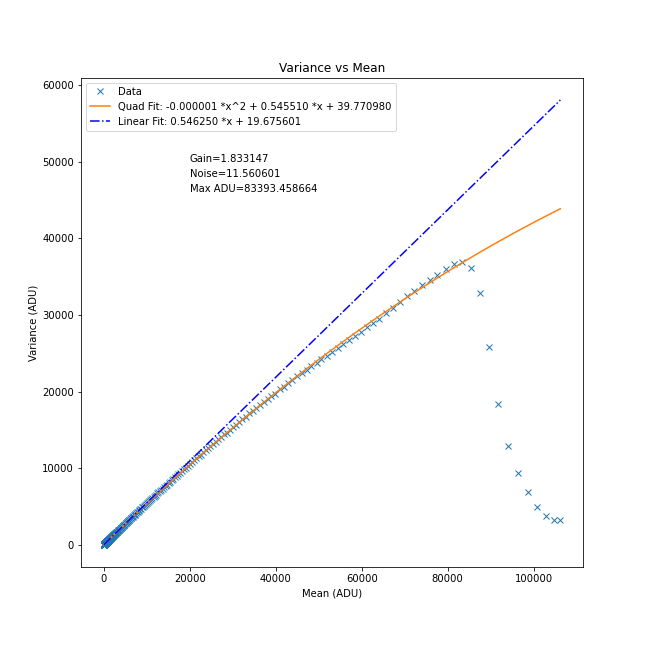
\includegraphics[width=0.6\columnwidth]{Plots/Plot1_Fit1.PNG}
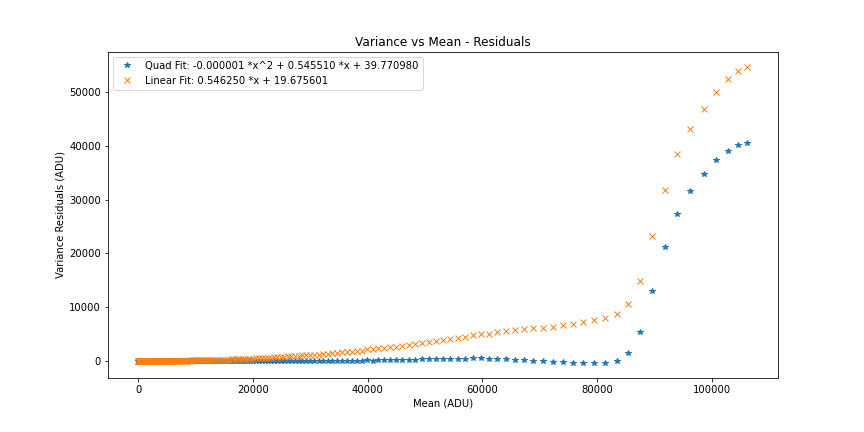
\includegraphics[width=0.6\columnwidth]{Plots/Plot1_Fit1_res.PNG}
\caption{\textit{Top: Quadratic and linear fit made with np.polyfit. Quadratic fit made using data points up to maximum variance. Linear fit made with points with $\mu<10000 \text{ ADU}$. Bottom: Residuals for both fits. }}
\label{plot1_fit}
\end{center}
\end{figure}

\begin{figure}[ht]
\begin{center}
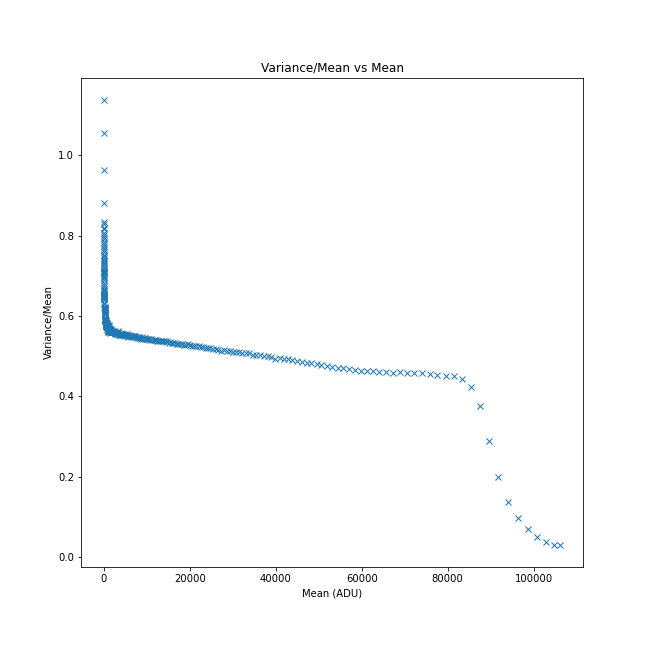
\includegraphics[scale=0.6]{Plots/var_muVSmu_1.PNG}
\caption{\textit{Variance (calibrated by the mean) vs mean for the first data set.}}
\label{varmuVSmu}
\end{center}
\end{figure}

By plotting the PTC (variance vs mean, fig. \ref{plot1_fit}) and its residuals from the fit model (see equation 16 from \cite{2019A&A...629A..36A}) wee see how the data presents higher absolute deviation more severely in the high flux regime. But if we plot the PTC normalized by the mean (fig. \ref{varmuVSmu}) we see how the low flux regime also presents high variances compared to the mean value obtained there. This is expected due to the effects of the reading noise of the detector which add randomness in the lectures for very low flux.

\vspace{5mm} %5mm vertical space

\subsection{ Task 2: Exploring Linearity with Diode Data.}\label{Diodes}

\noindent \textbf{Statement:} ``Here are the two files, one for each vendor.  Each one has the IDs of the exposure pair, the mean, the variance, the exposure time, and the monitor diode.  First, try plotting the monitor diode reading against the exposure time to see how linear this is.  Second, try plotting the mean against the monitor diode to see how linear the detector response is.  Since it will be quite linear, then try fitting the mean vs monitor diode with a straight line (linear fit) and plot the departure from the linear fit."

\noindent \textbf{Plots and fits:}

\noindent Figures \ref{diode1} and \ref{diode_fit} show the plots that resulted from solving task 2.

\begin{figure}[ht]
\begin{center}
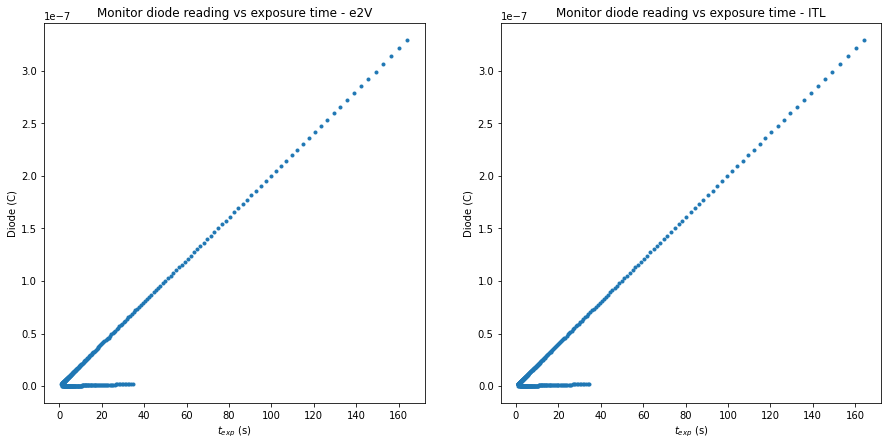
\includegraphics[scale=0.4]{Plots/t2p1.png}
\caption{\textit{Diode readings vs exposure time for two detectors, one E2V and one ITL. The expected linearity is noted.}}
\label{diode1}
\end{center}
\end{figure}

\begin{figure}[ht]
\begin{center}
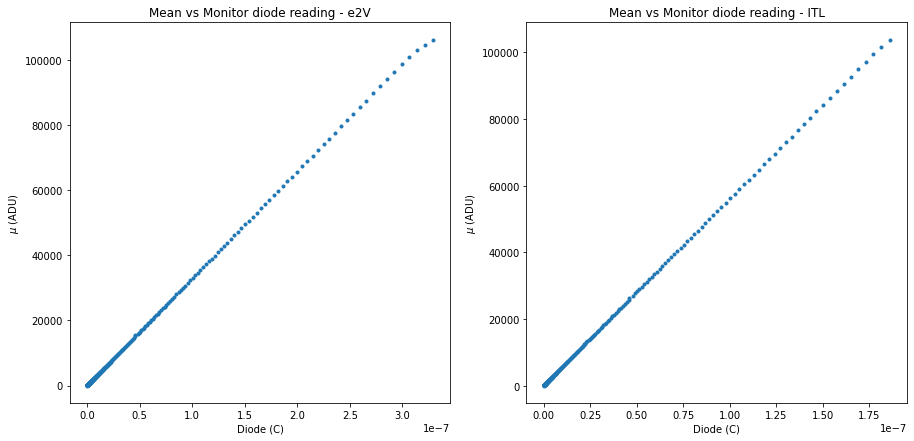
\includegraphics[scale=0.4]{Plots/t2p2.png}
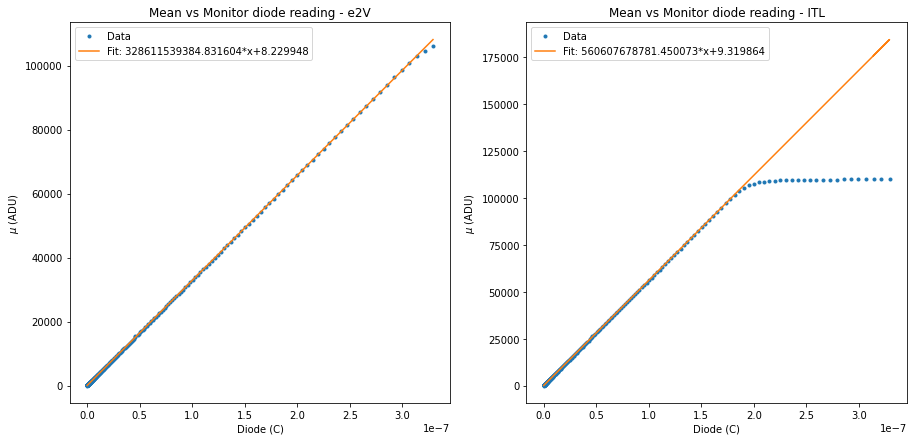
\includegraphics[scale=0.4]{Plots/t2p3.png}
\caption{\textit{Mean intensity values vs diode readings for both detectors without and with linear fits until linearity is lost.}}
\label{diode_fit}
\end{center}
\end{figure}

In this task we can see how \textbf{diodes are flux calibrators} to check the response of the detectors, since the monitor diodes measure flux by getting charged under a well-known linear behavior. In figures \ref{diode1} and \ref{diode_fit} we see how the linear regime ends when the detectors achieve fluxes of around 100000 ADUs, getting to the full well capacity of the pixels in the detector.\\

\vspace{5mm} %5mm vertical space

\subsection{ Task 3: Connection to RSP}\label{RSP}

\noindent \textbf{Cisco AnyConnect VPN Service:} NCSA requires connection through the Cisco AnyConnect VPN. Installation can be achieved easily by downloading the installer from the webpage: \href{https://its.gmu.edu/knowledge-base/how-to-install-cisco-anyconnect-on-linux/}{https://its.gmu.edu/knowledge-base/how-to-install-cisco-anyconnect-on-linux/} (Linux) or \href{https://its.gmu.edu/knowledge-base/how-to-install-cisco-anyconnect-on-a-windows-computer/}{https://its.gmu.edu/knowledge-base/how-to-install-cisco-anyconnect-on-a-windows-computer/} (Windows).\\

\noindent After installation one must connect to the NCSA server as shown in figure \ref{cisco}. Make sure you are connecting to ``NCSA SSLVPN" with the group ``ncsa-vpn-default", with your assigned NCSA username and password. For second password you can type ``push" to get sent a push notification through the Duo App or type in one of your Duo Passcodes (set a Duo account linked to your NCSA account if you have not done it already:
\href{https://wiki.ncsa.illinois.edu/display/cybersec/Duo+at+NCSA}{https://wiki.ncsa.illinois.edu/display/cybersec/Duo+at+NCSA} ).\\

\begin{figure}[ht]
\begin{center}
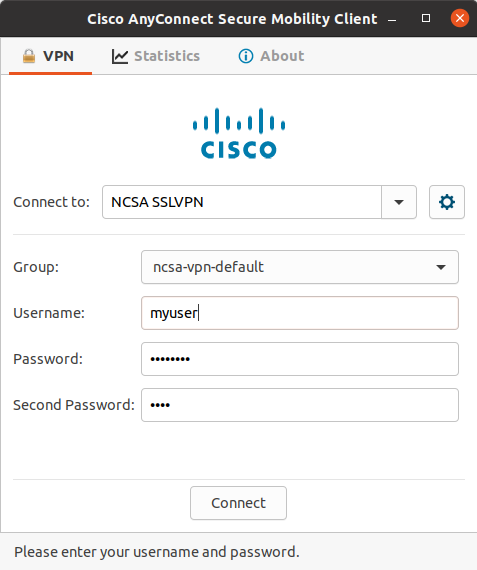
\includegraphics[scale=0.4]{Plots/CISCOANYCONNECT.png}
\caption{\textit{Cisco Anyconnect GUI.}}
\label{cisco}
\end{center}
\end{figure}

\noindent After aproving connection via the Duo push notification (or Duo passcode) the status of the VPN should appear as ``Connected".\\

\noindent \textbf{RSP:} To access the Rubin Science Platform follow the link: \href{https://lsst-lsp-stable.ncsa.illinois.edu/}{https://lsst-lsp-stable.ncsa.illinois.edu/}, you should get the page shown in figure \ref{rsp1}, there we only have access to the ``Notebooks" section, which will let us work with Notebooks, Terminals and files that we have in our user folder and the main directories.

\begin{figure}[ht]
\begin{center}
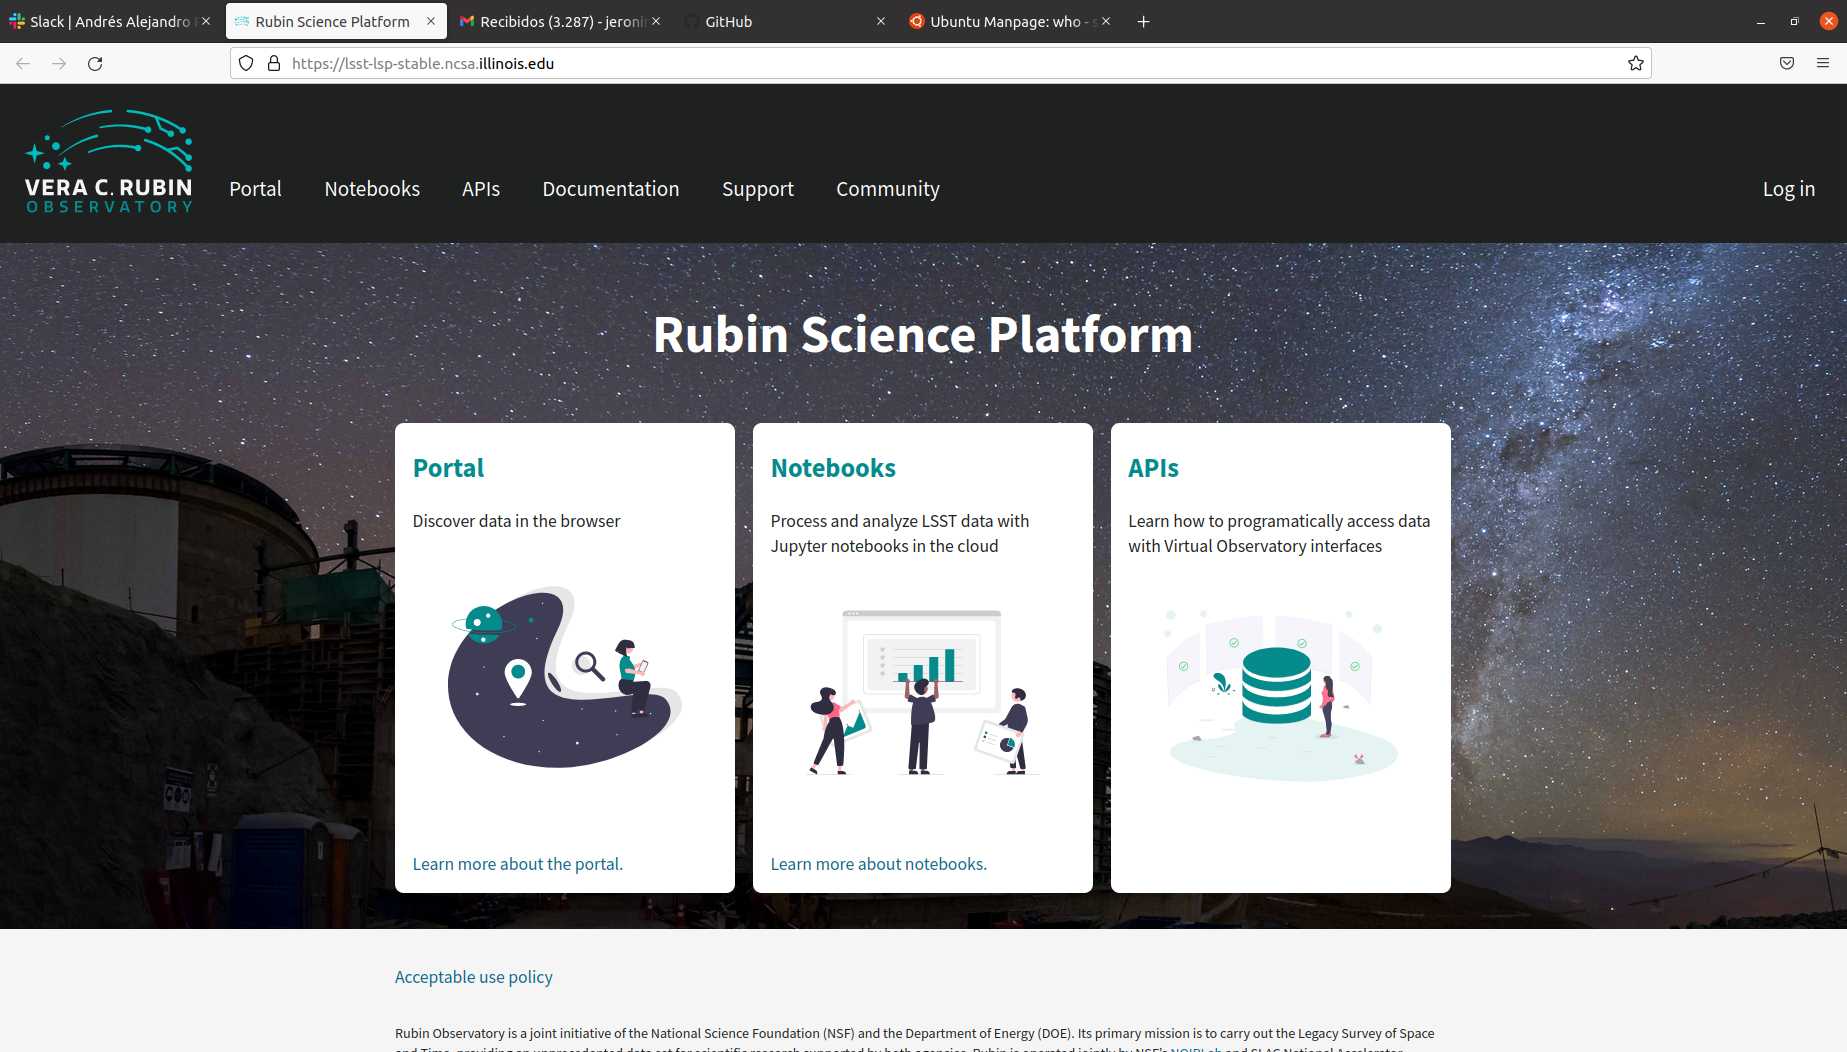
\includegraphics[scale=0.15]{Plots/RSP1.png}
\caption{\textit{Rubin Science Platform login page. Here we only have access to the ``Notebooks" section.}}
\label{rsp1}
\end{center}
\end{figure}

\noindent \textbf{Via SSH:}

\begin{enumerate}
    \item Login to NCSA through one of the servers: \\
    \texttt{ssh myuser@141.142.181.16\\
lsst-login01.ncsa.illinois.edu\\
lsst-login02.ncsa.illinois.edu\\
lsst-login03.ncsa.illinois.edu}
    \item Login as dev:\\
    \texttt{ssh lsst-devl01.ncsa.illinois.edu}
    \item Load LSST: \texttt{. /software/lsstsw/stack3/loadLSST.bash}
    \item Setup: \texttt{setup lsst\char`_distrib}
    \item Create yaml file for authentication, this is done with a text editor like nano or vi in the folder: \texttt{/home/USER/.lsst/db-auth.yaml} \\
    \texttt{- url: "postgresql://lsst-pg-prod1.ncsa.illinois.edu:5432/lsstdb1"\\
              username: "myuser"\\
              password: "mysecretpasswd"}\\
              Check that the words ``username" and ``password" are aligned with the ``u" in ``url". Keep the dash in the beggining.
    \item Data example: \\
    \texttt{pipetask run -j 32 -d "detector IN (0) AND instrument='LATISS' AND exposure IN \\(2022050500251..2022050500290) AND exposure.observation\char`_type='flat'" -b /repo/main -c isr:doFlat=False -i LATISS/raw/all,LATISS/calib -o u/jcalderong/test.1 -p\\ \$CP\char`_PIPE\char`_DIR/pipelines/Latiss/cpPtc.yaml --register-dataset-types}\\
    This runs for a couple of minutes and creates the file `test.1'.

    \begin{figure}[ht]
    \begin{center}
    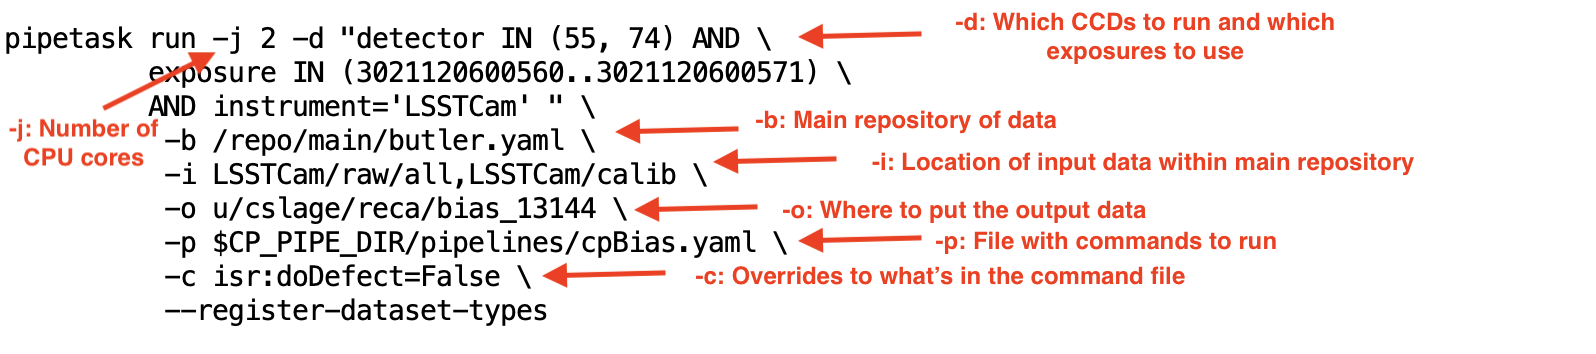
\includegraphics[width=0.8\textwidth]{Plots/pipetask.png}
    \caption{\textit{Explanation of the pipetask commands.}}
    \label{pipetask}
    \end{center}
    \end{figure}

\end{enumerate}
